\chapter*{Fasi per il riconoscimento della posizione all'interno degli edifici}
L'identificazione della posizione all'interno di un edificio si svolge in 2 fasi:
\begin{enumerate}
	\item Scansione dell'ambiente
	\item Ricerca della posizione
\end{enumerate}

\section*{Scansione dell'ambiente}
Analisi statica dell'ambiente chiuso, nel quale il software raccogliera' le onde magnetiche per ogni intervallo di tempo, le classifichera' con una semplice label la quale rappresentera' la zona di appartenenza.\\
La scansione a sua volta composta da diverse sotto-fasi cio\`{e}:
\begin{enumerate}
	\item Raccoglimento dei dati
	\item Estrazione del magnitudo
	\item Raggruppamento
	\item Estrapolazione delle \textit{features}
\end{enumerate}
\newpage
\subsection*{Raccoglimento dei dati}
Innanzitutto esaminiamo la composizione dei dati che stiamo andando ad estrarre: si tratta di onde magnetiche quindi strutturate nel seguente modo:\\
\begin{center}
	$(x,\, y,\, z)$
\end{center}
I tre valori sono espressi in $ \mu T $ (micro Tesla), unita' di misura della densita' di un flusso magnetico. Ad ogni onda magnetica viene assegnata una \textit{label}: una stringa od un numero che identifica univocamente una parte dell'ambiente chiuso
\begin{figure}[H]
\centering
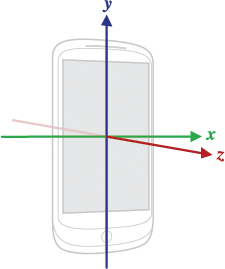
\includegraphics[width=0.20\linewidth]{./img/axis_magnetic_field.png}
\caption{Raffigurazione grafica delle onde raccolte}
\label{fig:axis_magnetic_field}
\end{figure}

\subsection*{Estrazione del magnitudo}
Per estrarre l'intensit\`{a} di ogni onda magnetica eseguiamo semplicemente la norma euclidea di un vettore:\\
\begin{center}
	$ \sqrt{x^2 + y^2 + z^2}$
\end{center}

\subsection*{Raggruppamento}
Le onde magnetiche con la stessa \textit{label} vengono raggruppate in \textit{fingerprints}, insiemi di dimensione prefissata. A livello logico, ogni \textit{fingerprint} cerca di identificare univocamente un punto all'interno di una zona, identificata con una \textit{label}. L'insieme di \textit{fingerprints} quindi, cerca di distinguere, tramite le caratteristiche dei campi elettromagnetici di ciascun punto, ogni \textit{label} dall'altra.

\subsection*{Estrapolazione delle \textit{features}}
Per ogni \textit{fingerprint}, l'estrazione delle \textit{features} consiste nell'estrazione di variabili statistiche. In questo specifico caso sono:
\begin{itemize}
	\item Media
	\item Varianza
	\item Deviazione standard
	\item Mediana
	\item Media troncata
	\item Coefficiente di variazione
	\item Massimo
	\item Minimo
	\item $ 1^{\circ}, 5^{\circ}, 95^{\circ}, 99^{\circ} $ percentile
	\item $ 1^{\circ}, 2^{\circ}, 3^{\circ} $ quartile
\end{itemize}



\section*{Ricerca della posizione}
Dopo aver scansionato l'ambiente questa fase viene eseguita dal cliente durante l'utilizzo dell'applicazione. La ricerca consiste nel creare sul momento una \textit{fingerprint} e poi, tramite un algoritmo di apprendimento automatico, cercare di inferire la \textit{label}  su cui ci troviamo. Nello specifico, l'algoritmo utilizzato e' il \textit{k nearest neightbours}.
\newpage

\section*{Apprendimento supervisionato}
Gli algoritmi di apprendimento usati rientreranno tutti sono la categoria di apprendimento supervisionato, quindi dovremo fornire degli esempi con un valore associato. In termini piu' formali si parla di un insieme di addestramento \textbf{X}, \textbf{y} dove $\forall x_i \in \textbf{X},\,\,x_i$ e' un insieme di attributi mentre $y_i \in \textbf{y}$ rappresenta il valore associato a quell'insieme di attributi.\ Quest'ultimo puo' essere discreto che continuo: nel primo caso si parla di classificazione mentre nel secondo di regressione.\\

\section*{K-nearest-neightbours}
Uno degli algoritmi piu' semplici di apprendimento automatico, e' il \textit{k-nearest-neightbours} dove l'input consiste in $k$ elementi presi dal \textit{training set} piu' vicini in base ad un criterio scelto da chi utilizza l'algoritmo (per esempio la distanza euclidea o di Mahalanobis).


\begin{figure}[H]
	\centering
	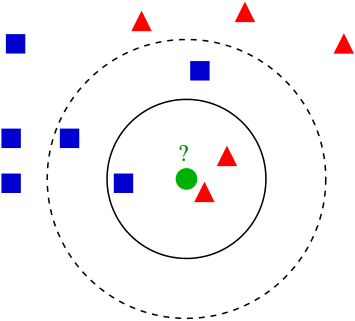
\includegraphics[width=0.7\linewidth]{img/knn_example}
	\caption{Esempio grafico dell'algoritmo KNN}
	\label{fig:knnexample}
\end{figure}


\subsection*{Scelta del parametro k}
La scelta del parametro dipende, ovviamente, dal tipo dei dati che abbiamo e dalla quantita', anche se in generale piu' e' grande $k$ meno rumore viene generato da questo algoritmo. Un buon metodo per trovare il giusto valore e' l'uso di tecniche euristiche, come la \textit{cross validation}. Un altra fonte di rumore di cui bisogna stare attenti e' la presenza di \textit{features} insignificanti nella ricerca del vicino. Per porre rimedio possiamo, ad esempio, usare un algoritmo genetico per selezionare le \textit{features} piu' significative

\subsection*{Cross validation}
Tecnica per migliorare le performance di un classificatore, consiste nel suddividere l'intero \textit{dataset} in $n$ parti uguali (di solito 10), ognuna delle quali svolgera' per una volta il ruolo di \textit{validation set} mentre il resto sara' il \textit{training set}. Questa tecnica risolve vari problemi tra i quali l'\textit{overfitting}.\\

\section*{Naive bayes}
Un altro tipo di apprendimento usato per classificare le \textit{label} e' Naive bayes: un algoritmo di classificazione e regressione basato sulla statistica. Prima di spiegare in cosa consiste occorre spiegare un paio di concetti:
\subsection*{Teorema di bayes}
: esso si fonda sul famoso teorema di bayes enunciato come segue:
\begin{center}
	$P(B|A) = \dfrac{P(A|B)P(B)}{P(A)}$
\end{center}
\subsection*{Rete bayesiana}
Una rete bayesiana e' un grafo diretto aciclico i cui nodi rappresentano le variabili casuali del sistema mentre gli archi rappresentato la condizione di dipendenza fra nodi.
 Ad ogni nodo e' associata una tabella di distribuzione delle probabilita' la cui complessita' e' proporzionale al numero di archi entranti.\\ Per esempio se il nodo con variabile casuale Leggere ha un arco verso Istruito allora possiamo dire che Istruito e' condizionalmente dipendente da Leggere. Qui sotto potete vedere una raffigurazione grafica di una semplice rete bayesiana formata da nodi padre ed un figlio:
\begin{figure}[H]
	\centering
	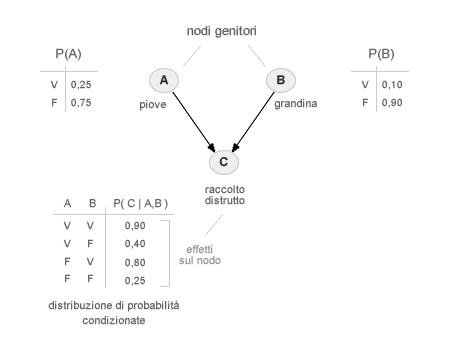
\includegraphics[width=0.7\linewidth]{img/rete-bayesiana-grafo.png}
	\caption{Esempio di rete bayesiana}
	\label{fig:rete-bayesiana-grafo}
\end{figure}
\medskip
\subsection*{Naive Bayes}
Naive bayes e' una rete bayesiana in cui si assume l'indipendenza condizionale fra tutte le variabili casuali del sistema data la classe. Questa forte assunzione non mira a modellare esattamente la realta' ma fornisce delle buone performance sulla predizione di una classe.

\begin{figure}[H]
	\centering
	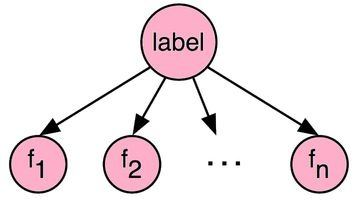
\includegraphics[width=0.4\linewidth]{img/naive_bayes_example}
	\caption{Esempio di rete bayesiana ingenua}
	\label{fig:naivebayesexample}
\end{figure}
\medskip
\subsection*{Un piccolo esempio basato su naive bayes}
Supponiamo di dover usare Naive Bayes per predire se giocare una partita di tennis o no in base alle condizioni meteorologiche. Dati gli esempi qui sotto a sinistra, possiamo ricavare la tabella di distribuzione delle probabilita' generale come qui di seguito:\\
\begin{figure}[H]
	\centering
	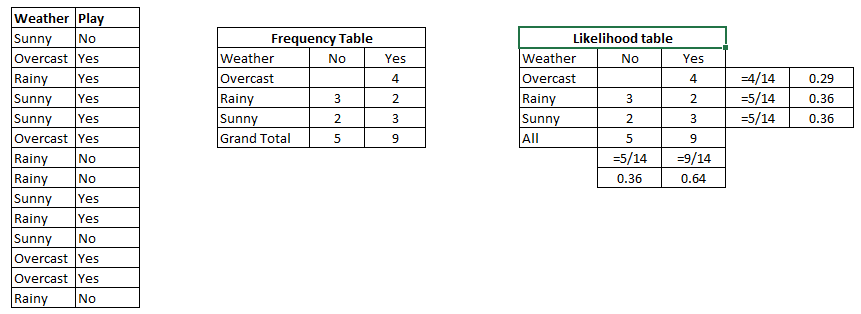
\includegraphics[width=0.7\linewidth]{img/Bayes_tennis_sample}
	\caption{Esempi di partite di tennis giocate in base alle condizioni meteorologiche e tabella di distribuzione delle probabilita'}
	\label{}
\end{figure}
\medskip
Ecco una rappresentazione grafica di \textit{Naive Bayes}:\\\\
	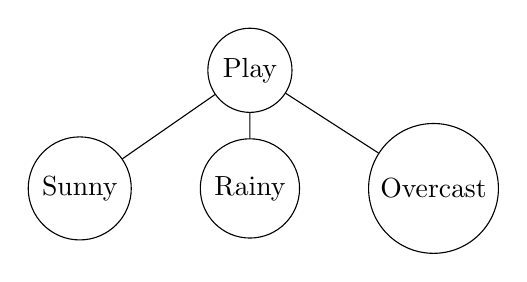
\begin{tikzpicture} 
		\node[draw, circle](0){Play}
		child{ node(1)[draw, circle, left]{Sunny}}
		child{	 	node(2)[draw, circle]{Rainy}}
		child{	  node(3)[draw, circle, right]{Overcast} };
	\end{tikzpicture}
\section*{Alberi di decisione}
Gli alberi di decisione sono un altro tipo di apprendimento supervisionato, quindi dovremmo avere 
Da un punto di vista strutturale, l'albero di decisione e' un albero (inteso come struttura dati) dove i nodi interni sono gli attributi, i rami tutti i possibili valori assumibili dall'attributo (oppure un range nel caso continuo) e le foglie sono la predizione da scegliere\\D'ora in poi parleremo, per semplicita', solo di classificazione quando non espresso chiaramente.
\subsection*{Costruzione di un albero di decisione}
L'albero di decisione si potrebbe definire prendendo a caso un attributo ed iniziare a dividere gli esempi fino ad ottenere foglie, anche se cosi' otterremo un albero  non molto utile in tutti i casi in cui non abbiamo gli esempi. Quindi quale albero scegliere fra tutti quelli possibili? In questo caso ci aiuta il rasoio di Occam, che ci dice di scegliere quello piu' piccolo fra tutti. Per generare l'albero piu' piccolo dovremmo scegliere gli attributi piu' significativi per generare l'albero. Cosa intendiamo per significativo? Intendiamo l'attributo che genera figli con meno varieta' di classi presenti all'interno di essi.\\ Un esempio: immaginiamo di avere 10 esempi con attributi A e B e come valore associato un booleano. se abbiamo l'attributo A che genera due figli con esempi aventi meta' valore vero e falso mentre se suddividiamo secondo B abbiamo figli con esempi esclusivamente veri oppure falsi. In questo caso indubbiamente l'attributo piu' significativo e' B.
\subsection*{Classificazione dei nuovi elementi}
Quando dovremmo predire l'etichetta di un nuovo insieme di attributi $x$ bastera' semplicemente scorrere l'albero di decisione dalla radice fino ad una foglia, che sara' l'etichetta da assegnare.
\subsection*{Un esempio di albero di decisione}
Riprendiamo l'esempio della partita di tennis, questa volta con qualche attributo in piu'. La tabella e' la seguente:
\begin{figure}[H]
	\centering
	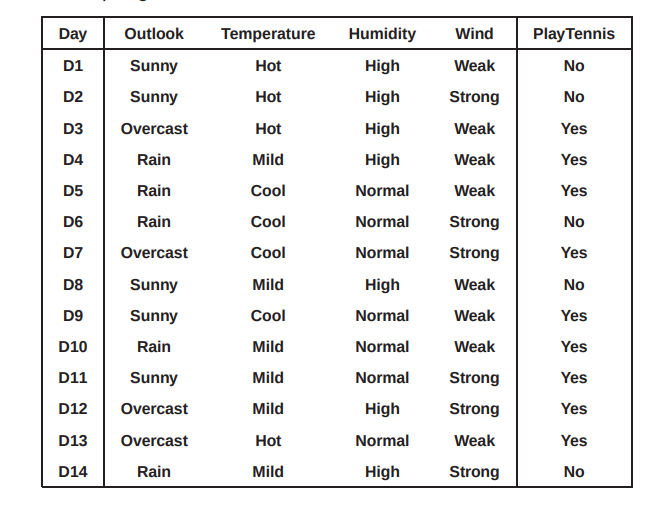
\includegraphics[width=0.7\linewidth]{img/decision-_tree_table_tennis}
	\caption{Tabella degli attributi meteorologici con valore associato un booleano che stabilisce se la partita e' stata giocata o no}
	\label{fig:decision-treetabletennis}
\end{figure}
da cui possiamo ricavare il seguente albero di decisione:
\begin{figure}[H]
	\centering
	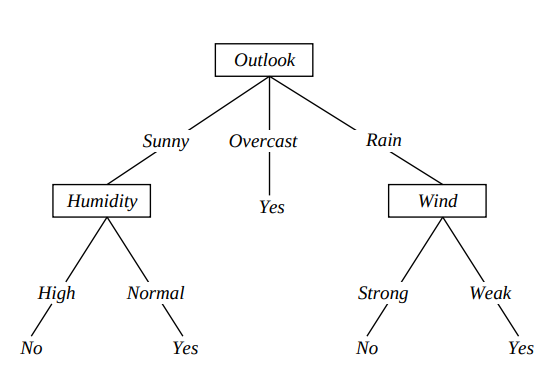
\includegraphics[width=0.7\linewidth]{img/decision_tree_tree_tennis}
	\caption{Albero di decisione ricavato dalla tabella precedente}
	\label{fig:decisiontreetreetennis}
\end{figure}


